\documentclass[heading.tex]{subfiles} 
\begin{document}

% \tableofcontents

\section{Background and Motivation}
Historically, there have been completely separate code-bases for design space exploration and transient engine analysis. The capability to create flexible "low fidelity" models is ideal in the earliest  conceptual design stages, where large design spaces can be explored relatively quickly. As the engine design starts to become more concrete, higher fidelity models are developed. These higher detail models are intrinsically more sensitive to design tweaks, and in general take longer to setup. They inherently require more stringently defined sets of boundary conditions and a specific configuration. A large variation in the baseline design could potentially render entire higher fidelity analyses obsolete. Due to this weakness in adaptability, higher fidelity models are generally not created until the low-fidelity design has fully matured. This friction can partly be attributed to the differences in toolstes when transitioning to higher fidelity models. 

\section{Introduction}
\subsection{Design Cycle Overview}

In the conceptual study phase of a typical design process, the engine is simulated in a few models of varying fidelity. “Low fidelity” models are ideally suited early on, due to their flexibility to explore the entire design space, and their relatively short setup time. As the engine design starts to become more concrete, higher fidelity models are developed. These higher detail models are intrinsically more sensitive to design tweaks, and in general take longer to setup. They inherently require more stringently defined sets of boundary conditions and a specific configuration. A large variation in the baseline design could potentially render entire higher fidelity analyses obsolete. Due to this weakness in adaptability, higher fidelity models are generally not created until the low-fidelity design has fully matured. 
	From a life-cycle cost perspective, there comes a point when the prospect of re-design becomes prohibitively expensive and initial design decisions become cemented into the design.  Any insights gained from more detailed analyses are constrained to these initial design choices. Naturally, a tradeoff exists on the amount of time spent in each analysis phase. Spending more time in the low fidelity phase could have large payoffs in the long run; however, without higher fidelity models it is hard to identify possible shortcomings such as those arising from operability and control issues.

\begin{figure}[hbtp]
\centering
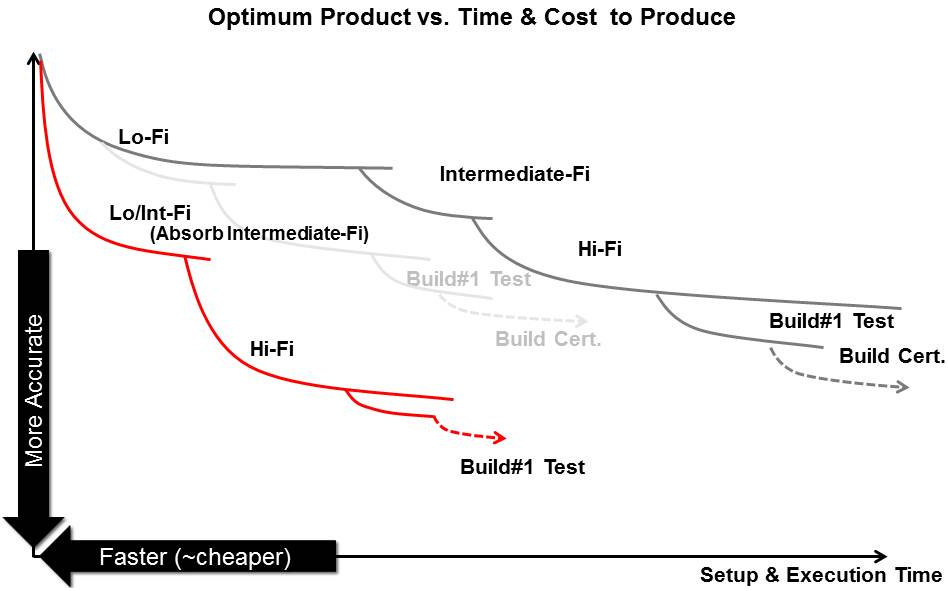
\includegraphics[width=1.0\textwidth]{images/optimum_product_vs_time}
\caption{Overarching Applied Research Challenge: Uncertainty in Optimum Product vs. Time \& Cost to Produce}
\label{f:product_vs_time}
\end{figure}


Figure 1 shows a pedagogical representation of the general relation between accuracy and analysis set-up time. Lower fidelity  models are less accurate, but can be set up and modified relatively quickly. The darker gray path characterizes the tradtional design trend. Higher fidelity models take longer to build, and therefore, aren’t started until the low fidelity model nears completion. If designers attempt to introduce Hi-Fi models earlier in the design, (as shown by the light gray line shifted to the left) they quickly become outdated as the baseline model continues to undergo changes. Inevitably the models must be re-written to match the new Lo-Fi design and the path reverts to the dark gray route. The only way to incorporate the intermediate fidelity model earlier into the design process, is by absorbing the Int-Fi codes into the low fidelity codes as portrayed by the red line. Combining both codes into a unified code would acomplish this, but the codes can also be kept distinct as long as the Int-Fi model is adaptible enough to keep up with the rapid changes of the Low-Fi code. Creating a single unified code can potentially become complex and cumbersome. A natural reaction is for various disciplines to diverge and create unique tools satisfying their particular needs using frameworks and programming languages already of familiarity. As mentioned earlier, this is acceptable and still “unifiable” as long as the codes preserve flexibility and rapid adaptability. An intermediate fidelity code can be introduced earlier into the low fidelity analysis phase if it can keep pace with the rapid redesigns.
	In the context of NASA Glenn’s supersonic program, the Numerical Propulsion System Simulation (NPSS) VCE engine is the low fidelity model, and the Supersonic Component Engine Model (SCEM) is the intermediate fidelity model. The NPSS model is a framework written in C++, while the SCEM model is developed within the Matlab/Simulink environment. The SCEM model performs its own unique calculations, but requires the steady-state engine characteristics of the NPSS model to initialize the simulation. Large advances needed to be made to the intialization scripts of the SCEM program if both programs are to be run congruently. A brief history of the SCEM model is provided below to shed light on the amount of work that is required to build such a model and to emphasize the clear need for improved extensibility.  

\section{Volume Dynamics}
\subsection{Background}
Under the NASA Fundamental Aeronautics Program, the Supersonics Project is developing a variable cycle engine (VCE) model for use in aero-propulso-servo-elastic (APSE) coupling studies of supersonic vehicles. (Connolly, Kopasakis, \& Lemon, 2010) Analytical, computational, wind tunnel and flight data of Aero-Servo-Elastic (ASE) systems have been thoroughly vetted however much work still needs to be done to integrate propulsion dynamics into the ASE analysis tool suite. (Fundamental Aeronautics Program Supersonics Project, 2006)
The Controls \& Dynamics branch and the Multidisciplinary Design, Analysis \& Optimization (MDAO) branch at NASA Glenn are working in conjunction to produce a propulsion model that will eventually be of a sufficient fidelity to directly couple with full-scale computational fluid dynamic (CFD) and structural dynamic models. The task has been partitioned into three connected simulations: a two-dimensional bifurcated inlet, a variable cycle turbofan engine, and variable area exit nozzle. (Connolly, Kopasakis, Paxson, Stuber, \& Woolwine, 2012) 
Development of the engine simulation has proven difficult, largely due to the number of components involved. Many of the challenges have been associated with data management issues or difficulties in adaptability as the simulation has been scaled up in fidelity and engine complexity. The main intent of this report is to discuss the strategies used to construct and initialize these large models.  The methodology for computing component performance has been adopted from previous work completed by the Controls \& Dynamics group, (Kopasakis, Connolly, Paxson, \& Ma, 2008) and is beyond the scope of this paper.
This report focuses on a novel software generation tool being designed to dramatically reduce engine model set-up time, allowing higher fidelity analyses to be introduced earlier in the design cycle. The software is intended to work for any type of engine architecture, but was originally tailored for the VCE configuration. The benefits of the tool are most apparent when its impacts are framed from a design cycle standpoint.

\section{Conclusions}
This is conclusions section it's quite handy.


\end{document}

%%% Local Variables: 
%%% mode: latex
%%% TeX-master: t
%%% End: 
